%Note one sentence in one text line.
\section{Traffic Redirection to Monitor Mobile Internet Traffic} 
\label{sec:platform} 

\tbd{Should we explicitly mention traffic redirection as a tool?}
In this section, we first detail our goals. 
We then show that traffic redirection can be used to achieve our described goals in a feasible manner. 

\subsection{Goals}  
\label{sec:goals} 
Our primary goal is \emph{to monitor all the Internet traffic from mobile devices regardless of the operating system, wireless access technology, and the ISPs used by the mobile device}. 
%This comprehensive visibility is required to understand the Internet usage of  mobile devices and the ISP interference of mobile Internet traffic. 
We now present the following sub-goals we believe are essential to meet this goal.
\begin{packedenumerate}
\item \emph{Portable.} We want to maximize the number of OSes and brands that are included in measurement studies.  
\item \emph{Pervasive.} We want our measurements to be agnostic of the location, access technology, and ISPs used by mobile devices. 
\item \emph{Passive.} We want to monitor traffic even when the devices are \emph{idle}.
\item \emph{Deployable.} We want a low barrier to entry to ensure that end users can participate in our studies.
\end{packedenumerate}    
In summary, we define our goal using portability, pervasiveness, passiveness, and deployablity as its building blocks. 
\tbd{These points need to be revisited to incorporate Trip wires.}  

\subsection{Description}
\label{sec:description}

We now show that traffic redirection is the best way to reach our goals. 
We use two forms of redirection: a VPN based redirection to detail the network traffic characteristics of mobile device, and a transparent proxy based redirection to detail ISP interference of mobile Internet traffic. 

\subsubsection{VPN based Traffic Redirection} 

We were motivated to consider VPNs because corporate executives are known to connect to securely to their corporate servers using VPNs regardless of their location and available access technology.
The fact that corporate clients used VPNs gave us hints towards its portability and deployability.
We now show that VPNs can be pervasive and ideal to monitor mobile Internet traffic from end users.  

Android, BlackBerry, Bada, and iOS all support VPNs tunnels over Wi-Fi and the cellular interface.
All iOS devices (version 3.0 and above) come with a feature called ``VPN On-Demand''. 
\emph{VPN On-Demand} forces the iOS device to use VPN tunnels when connecting to a specified set of domains. 
Using trial-and-error, we discovered that VPN On-Demand uses suffix matching to determine which domains require a VPN connection. 
We use this knowledge to configure \emph{VPN On-Demand} such that iOS devices use a VPN tunnel to access the Internet. 
Android version 4.0 and above comes with native VPN support. 
Unlike iOS, Android does not offer an equivalent of \emph{VPN On-Demand}; however, Android provides an API that allows an user space app to manage VPN connections. 
We modify the open source StrongSwan VPN client~\cite{strongswanclient} to ensure that the VPN reconnects each time the preferred network changes (\eg, when a device switches from cellular to \wifi). 
As of Android 4.2, Android supports ``Always On'' VPN connections that uses VPNs to tunnel all the data traffic. 
\tbd{Dave:text on Always ON from inputs from Adrian}.

%We believe that a software based solution powered by open-source software is important. 
%Open source VPN solutions to manage VPN tunnels include Strongswan, Openswan, and OpenVPN.
\platname uses Strongswan~\cite{strongswan} because it is the only open source solution that can use the IPsec services of the Linux kernel \emph{without any kernel modifications}.
We emphasize on IPsec because the \emph{VPN On-Demand} feature of iOS is supported only for VPN tunnels that use IPsec and the IKEv1~\cite{rfc4109} key exchange protocol.
Furthermore, Strongswan also supports the faster IKEv2~\cite{rfc5996} key exchange protocol that is supported by Android clients.
%Thus Strongswan, which is used the IPsec services of the Linux kernel ensures that VPN tunnels can be managed using \emph{off-the-shelf} hardware and open source software.

\subsubsection{Redirection using a Transparent Proxy} 

\tbd{Dave add text here} 


\subsubsection{Traffic Monitoring Setup}

\begin{figure}
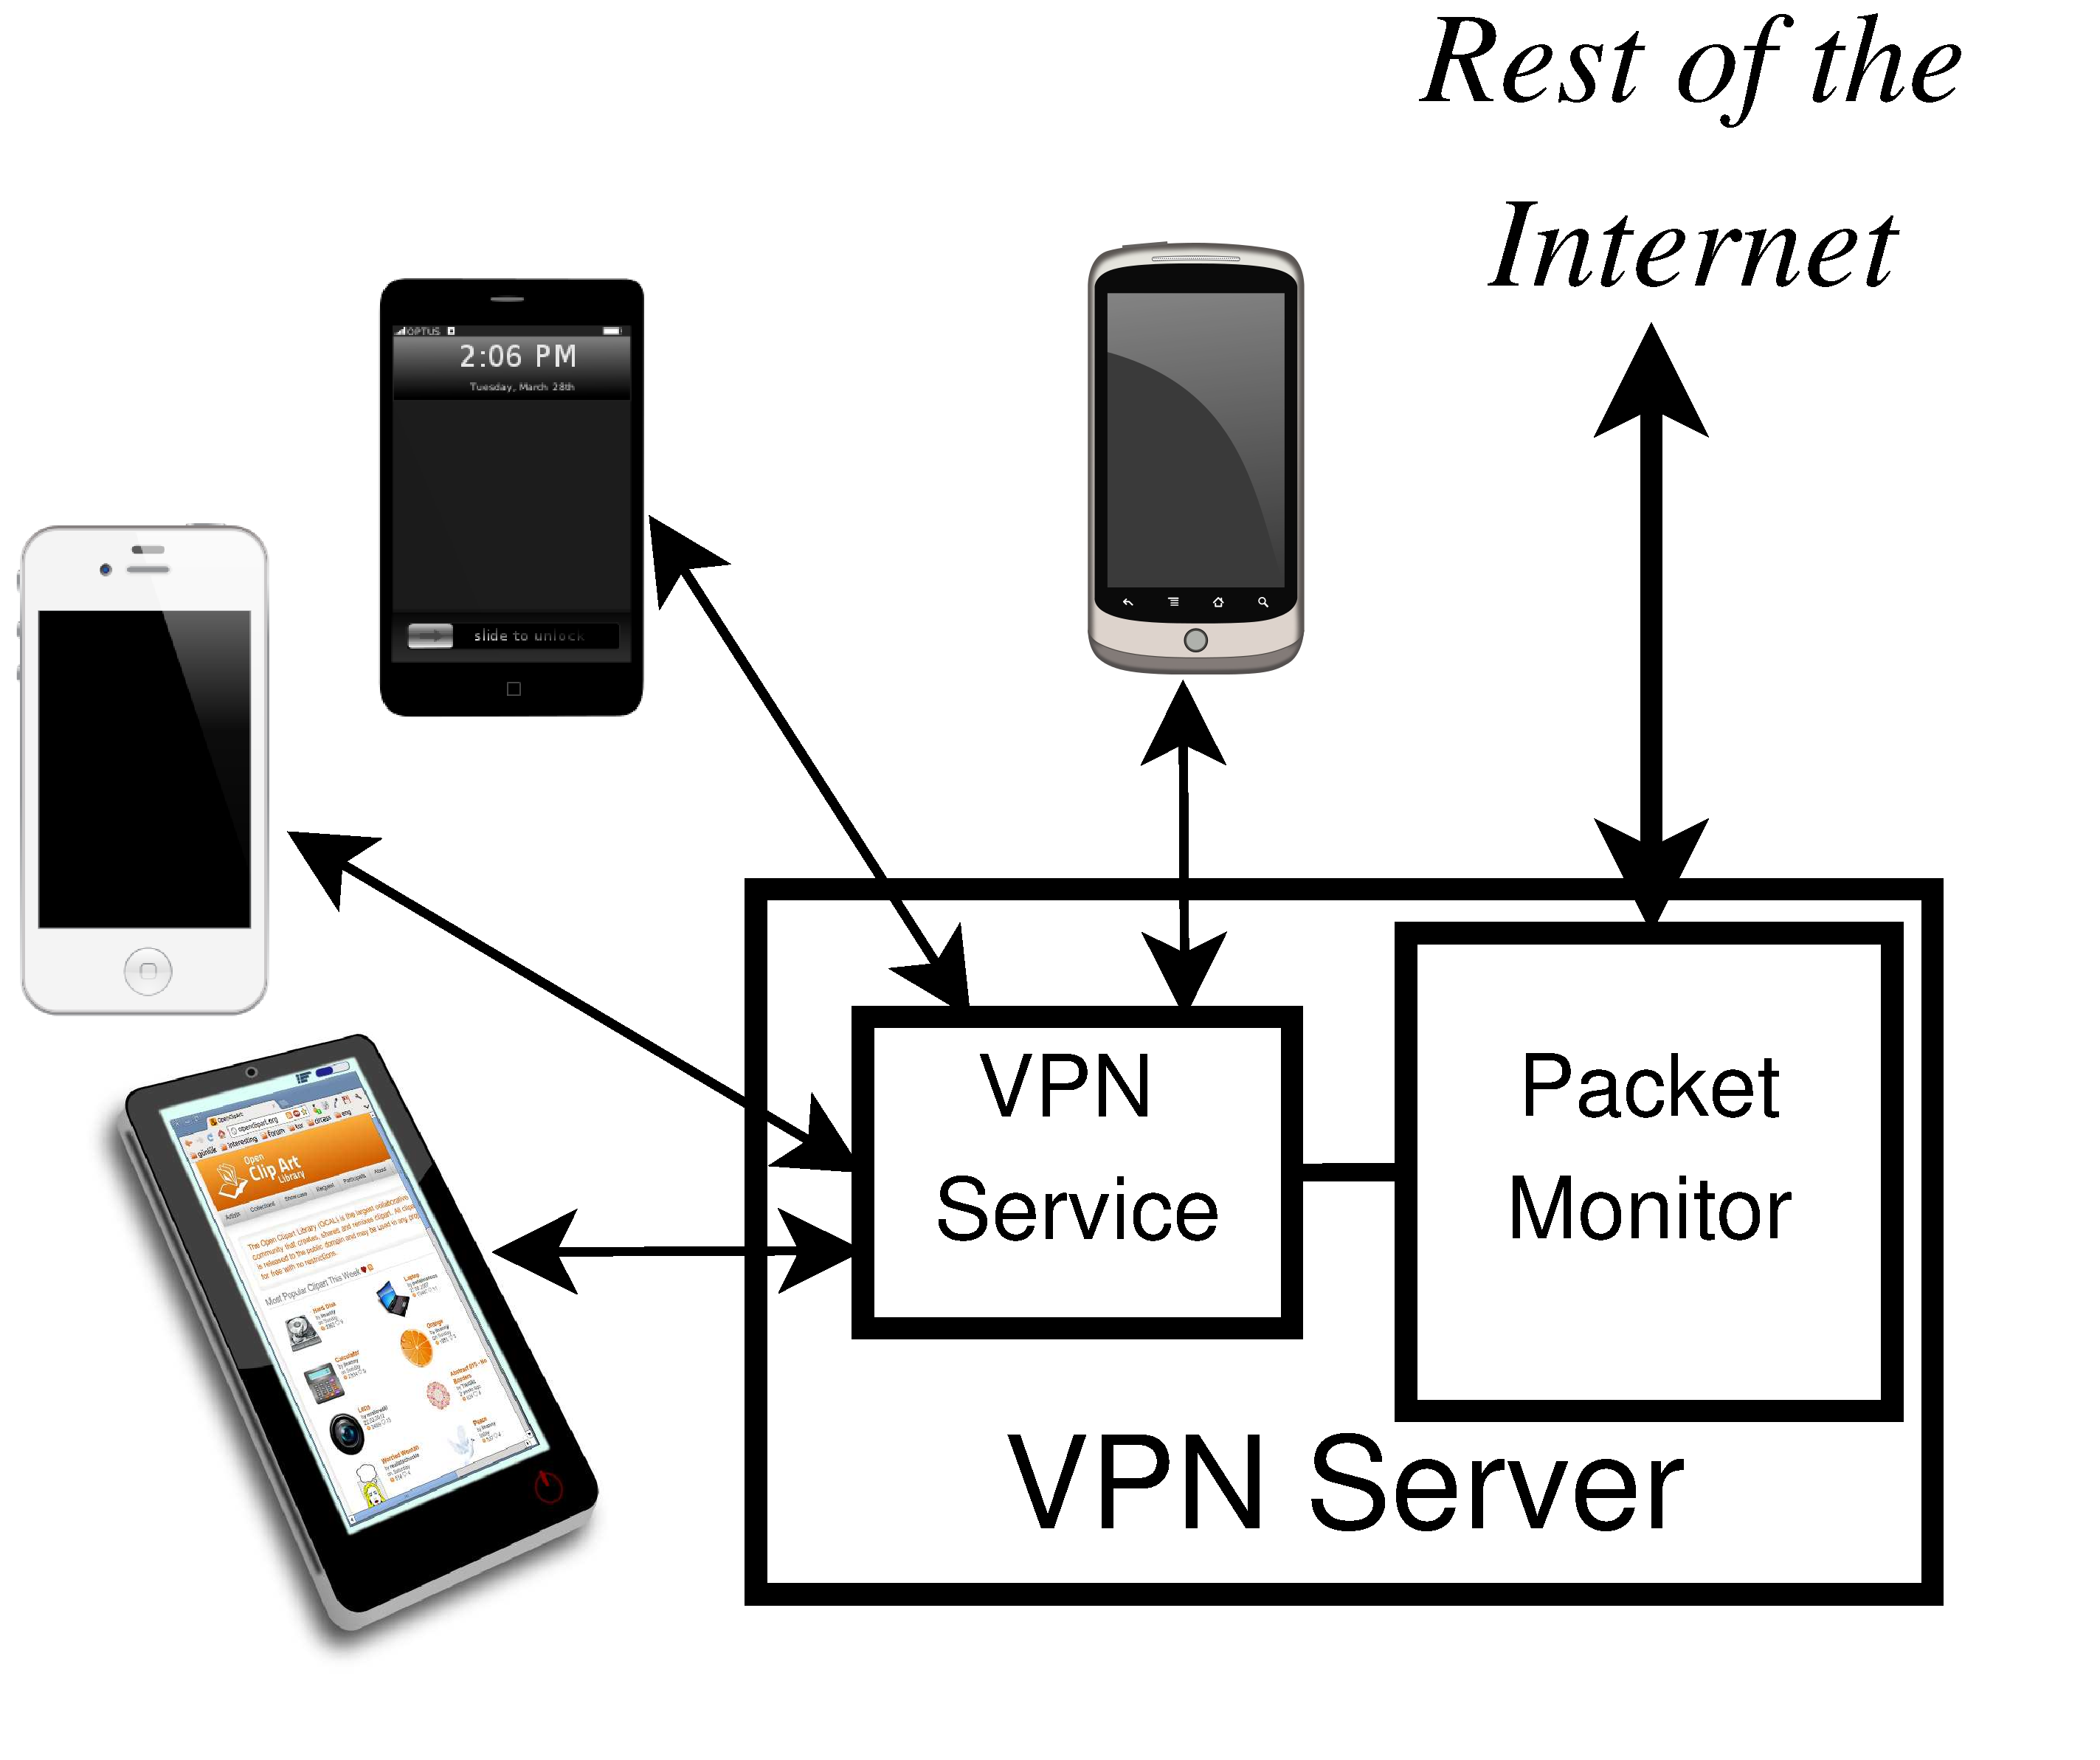
\includegraphics[width=\columnwidth]{figures/meddle-servers.pdf}
\caption{\platname uses traffic redirection to monitor mobile Internet traffic. \platname \emph{requires mobile clients to redirect their traffic through a server that monitors Internet traffic. VPN based redirection is used to characterize mobile traffic sans ISP interference. To detect ISP interference \platname relies on a single hop transparent Web Proxy.}}
\label{fig:description}
\end{figure}

As shown in \fref{fig:description}, mobile devices redirect their Internet traffic through a \platname server that monitors all their Internet traffic. 
VPNs are used to monitor all Internet traffic from mobile devices while a transparent Web proxy to detail interference by mobile ISPs.

Deploying VPNs on mobile clients is simple for end users primarily VPNs are natively supported by popular mobile OSes. 
The Android users need to install a certificate and fill our five fields while iOS users need to install a configuration file. 
Once the configurations are stored, all Internet traffic from the mobile device flows through \platname. 
\platname uses Strongswan to manage VPN tunnels of \platname.
This simplicity is important for practical and realistic measurement studies with end users.
We use tcpdump to monitor the traffic that passes through \platname servers.

\eat{ Remove text related to tun/tap device
We use tcpdump to monitor the packets that flowing through \platname. 
We now present the technique we used to segregate traffic from mobile devices. 
\platname uses NAT to divert the packets encapsulated in the VPN tunnels to Internet. 
In the ideal scenario, the encapsulated packets from the mobile device would be tunneled to \platname. 
On \platname, these packets would be decapsulated and the packets would then undergo NAT before leaving for their intended destination. 
The packets from the mobile clients to the Internet could be monitored before they undergo NAT.
However, due to the existing network stack implementation, the packets from the Internet that are destined to the mobile clients undergo NAT and IPSec encapsulation take place in one step.
The inter-dependencies between these various modules responsible for routing, NAT, and IPSec make it difficult segregate and monitor the packets. 
We address this issue by looping the packets through a virtual (\emph{tun/tap}) device. 
The looping of packets through a virtual device allows us to monitor the packets when they are outside the VPN tunnels and have not undergone NAT. 
}

\tbd{Dave: \fref {fig:tripnet} text for tripnet should come here}
\begin{figure}
\centering
\tbd{Dave: New figure for Tripnet comes here.} 
\caption{Overview of the Web tripnet }
\label{fig:tripnet}
\end{figure}


In summary, mobile VPNs are portable and deployable because they are natively supported by popular mobile operating systems.
We build on existing features provided by iOS and Android to make sure that the VPN tunnels are pervasive and are created passively. 
We rely on the open source Strongswan VPN daemon to manage VPN tunnels which makes \platname deployable.
We plan to release the source code to configure mobile Internet traffic using  \platname.

\subsection{Feasibility}

We now show that the cost to redirect traffic through \platname is low in terms of latency, data consumption, and power.

\subsubsection{VPN Latency Overheads }
The iOS devices use IKEv1 to manage the VPN tunnels while Android devices support both IKEv1 and IKEv2. 
To establish the VPN tunnel, IKEv1 requires a total 16 packets to be exchanged between the mobile client and the VPN server while IKEv2 requires 4 packets.
\platname uses IKEv2 for Android devices while IKEv1 is used for iOS devices. 

To measure the time required to establish a VPN tunnel, we performed controlled tests using one Android device and an iPhone 5. 
We performed these tests from two different locations based in the same city in which the server was deployed.
OUr tests involved \tbdv{number} of VPN tunnel creation over a time period of \tbdv{} hours. 
When the Android device used \wifi to establish the VPN tunnel, we observe a median connection establishment time of 0.62 seconds from both locations with a maximum of 0.81 seconds and 0.79 seconds respectively. 
When the Android device used cellular networks to establish the tunnel, the median connection establishment time was 0.81 seconds from both locations with a maximum of 1.59 seconds.
Compared to the Android device, the iOS devices required a larger amount of time to establish the connection because it relies on a an older key authentication protocol. 
From the two Wi-Fi networks, to establish the VPN tunnel, the iOS device required 1.60 seconds and 1.34 seconds with a maximum of 2.0 seconds and 1.48 seconds respectively; in the case of cellular networks  we observed a median of 1.80 seconds and 1.65 seconds with a maximum of 2.18 seconds and 1.87 seconds respectively. 

\tbd{In summary, we observe that because iOS devices use an older key exchange protocol they can take up to twice as much time as Android devices to establish the VPN tunnel. 
Any more insights .. The tunnel establishment times in the order of 2 seconds implies that \platname can have a significant latency overhead if VPN tunnels are established periodically for short tests.}

\subsubsection{Data Consumption Increase when using VPN}
IPSec encapsulation slightly inflates packet sizes, in addition to preventing carrier middleboxes from applying their own compression.
We measured the overhead of the tunnel in terms of data overhead from IPsec headers and keep-alive messages, finding that it
ranges from 8--12.8\%.

To to compute the increase in the amount of bytes transferred due to encapsulation and the keep-alive
messages, we log the packet lengths of the encrypted packets (IPsec packets) exchanged by our \platname servers and the mobile clients. 
We performed this packet capture for 30 days during which 25 devices tunneled their traffic via \platname. 
During this time interval we also log the packet length of the packets encapsulated within the IPsec packets. 
During this 30 day period we observe that the median of the increase to be 8.31\%, with a maximum increase of 12.8\%.

\tbd{In summary, we observe a maximum overhead of 12.8\% increase in data consumption. We believe the costs of this overhead are minimal compared to the cost of warrant voiding the device.}

\subsubsection{Power Overheads when using VPNs}
\tbd{Daves results}

\tbd{In summary, we show \platname is feasible to build and deploy}

\subsubsection{Impact of using Transparent Proxy}

\tbd{Dave: Text comes here}

\subsection{Discussion}

We now discuss some shortcoming of using traffic redirection
\begin{packedenumerate}
\item Traffic redirection implies that Web sites that use their clients IP addresses to offer custom services shall respond according the IP address of the \platname server. This can affect the quality of the results we observe in our datasets. 
\item Some ISPs are known to block VPNs. During our measurement we observed one such ISP that blocked VPN tunnel creation requests from one of our clients.
\item We observe that mobile devices currently create a VPN on at most one wireless interface. This implies that \platname shall not be able to monitor traffic when the mobile device simultaneously use more than one wireless interface. 
\item We performed controlled experiments to test IPv6 support. We observe that though iOS and Android support IPv6 they currently cannot tunnel IPv6 traffic through VPN tunnels. 
\item When using VPNs, \platname shall not be able to monitor the traffic between the mobile device and access point used to connect to the Internet.
\end{packedenumerate}

\tbd{In summary, despite these shortcoming we believe that \platname can be used for realistic measurements of mobile Internet traffic.}





